\documentclass[10pt]{standalone}
\usepackage{amsmath}
\usepackage{amssymb}
\usepackage{pgf,tikz}
\usepackage{mathrsfs}
\usetikzlibrary{arrows,calc}
\pagestyle{empty}
\usepackage{siunitx}
\begin{document}
	

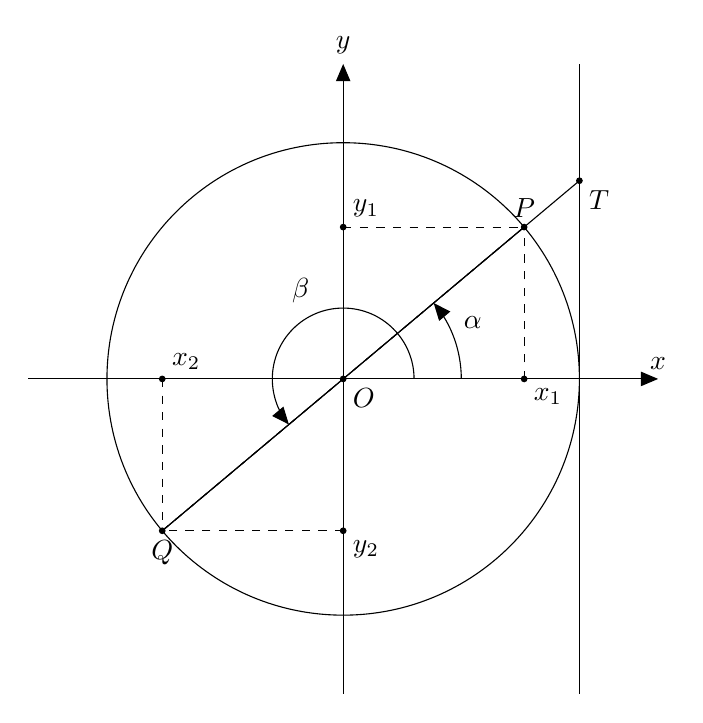
\begin{tikzpicture}[>=triangle  45]
\tikzset{samples=600}
\pgfmathsetmacro{\raggio}{3};
\pgfmathsetmacro{\angolob}{40};
\pgfmathsetmacro{\angolo}{\angolob};
\pgfmathsetmacro{\angolon}{\angolob+180};
\pgfmathsetmacro{\y}{3};
\pgfmathsetmacro{\xy}{5};
\pgfmathsetmacro{\XM}{\raggio};
\pgfmathsetmacro{\sraggio}{1.5*\raggio};
\coordinate [label=below right:$O$] (oo)  at (0,0);
\draw[->] (-\raggio-1,0) -- (\raggio+1,0) node[above] {$x$} ;
\draw[->] (0,-\raggio-1) -- (0,\raggio+1) node[above] {$y$} ;
\draw (\raggio,-\raggio-1) -- (\raggio,\raggio+1) ;
\draw (oo) circle (\raggio) ;
\coordinate[label=above:$P$] (P) at ({\raggio*cos(\angolo)},{\raggio*sin(\angolo)});
\coordinate[label=below:$Q$] (Q) at ({\raggio*cos(\angolon)},{\raggio*sin(\angolon )});
\coordinate[label=below right:$T$] (T) at (\raggio,{\raggio*tan(\angolon )});
%\coordinate [label=above left:$M$] (M) at ($((-\raggio,0)!(\angolo:\raggio)!(\raggio,0)$);
\coordinate[label=above right:$y_1$] (Y1) at (0,{\raggio*sin(\angolo)});
\coordinate[label=below right:$y_2$] (Y2) at (0,{\raggio*sin(\angolon)});
\coordinate[label=below right:$x_1$] (X1) at ({\raggio*cos(\angolo)},0);
\coordinate[label=above right:$x_2$] (X2) at  ({\raggio*cos(\angolon)},0);
\filldraw[black] (oo) circle(1pt);
%\filldraw[black] (M) circle(1pt);
\filldraw[black] (P) circle(1pt);
\filldraw[black] (Q) circle(1pt);
\filldraw[black] (T) circle(1pt);
\filldraw[black] (Y1) circle(1pt);
\filldraw[black] (Y2) circle(1pt);
\filldraw[black] (X1) circle(1pt);
\filldraw[black] (X2) circle(1pt);
\draw[dashed](Q)-- (P) ;
\draw[dashed](Y1)-- (P) ;
\draw[dashed](X1)-- (P) ;
\draw[dashed](Y2)-- (Q) ;
\draw[dashed](X2)-- (Q) ;
\draw[->] (\sraggio/\y,0 ) arc (0:\angolo:\sraggio/\y) ;
\draw (\angolo/2:\sraggio/\y) node[ above right]  {$\alpha$};
\draw[->] (\sraggio/\xy,0 ) arc (0:\angolon:\sraggio/\xy) ;
\draw (\angolon/2:\sraggio/\xy) node[above left]  {$\beta$};
\draw (oo)-- (P) ;
\draw (oo)-- (Q) ;	
\draw (T)-- (Q) ;
\end{tikzpicture}
\end{document}